|

\chapter{Resultados Obtidos}
\label{cap:resultados}
\glsresetall

Neste Capítulo serão mostrados os resultados referentes ao método discutido neste trabalho. Serão
apresentados a flutuação estatística das rede para cada uma das configurações testadas, a escolha do melhor número
de neurônios da camada escondida, o desempenho dos classificadores durante o treinamento e os resultados de 
eficiência e rejeição do classificador escolhido para operar no sistema de \textit{trigger} de alto nível do ATLAS.

\section{Dados Avaliados}

A seleção do conjunto de sinal formada pela seleção de elétrons extraidos dos dados simulados do decaimento $Z \rightarrow ee$ geraram
um total de 322407 eventos que serão utilizados para treinar o classificador. Para a seleção dos jatos, foram extraídos 11623 eventos
provenientes da simulação de jatos com $E_{T} > 17 GeV$. A seleção dos sinais respeitou as condições discutidas na Seção~\ref{sec:selecao_sinais} 
apresentadas no capítulo anterior. 

A Figura~\ref{fig:perfil_ringer} representa o perfil médio energético, medido em $MeV$, dos anéis para as amostras de elétrons do conjunto de $Z\rightarrow ee$ e de partículas hadrônicas pertencentes 
ao conjunto de jatos em $E_{T}>17 GeV$. Comparando os dois perfis de energia observa-se que as partículas hadrônicas excitam os anéis mais externos de cada camada além de liberar, em média, 
mais energia nas camadas hadrônicas. Assim, os jatos possuem um chuveiro mais largo e profundo que as interações dos elétrons no calorímetro. 

\begin{figure}[h!t]
\centering
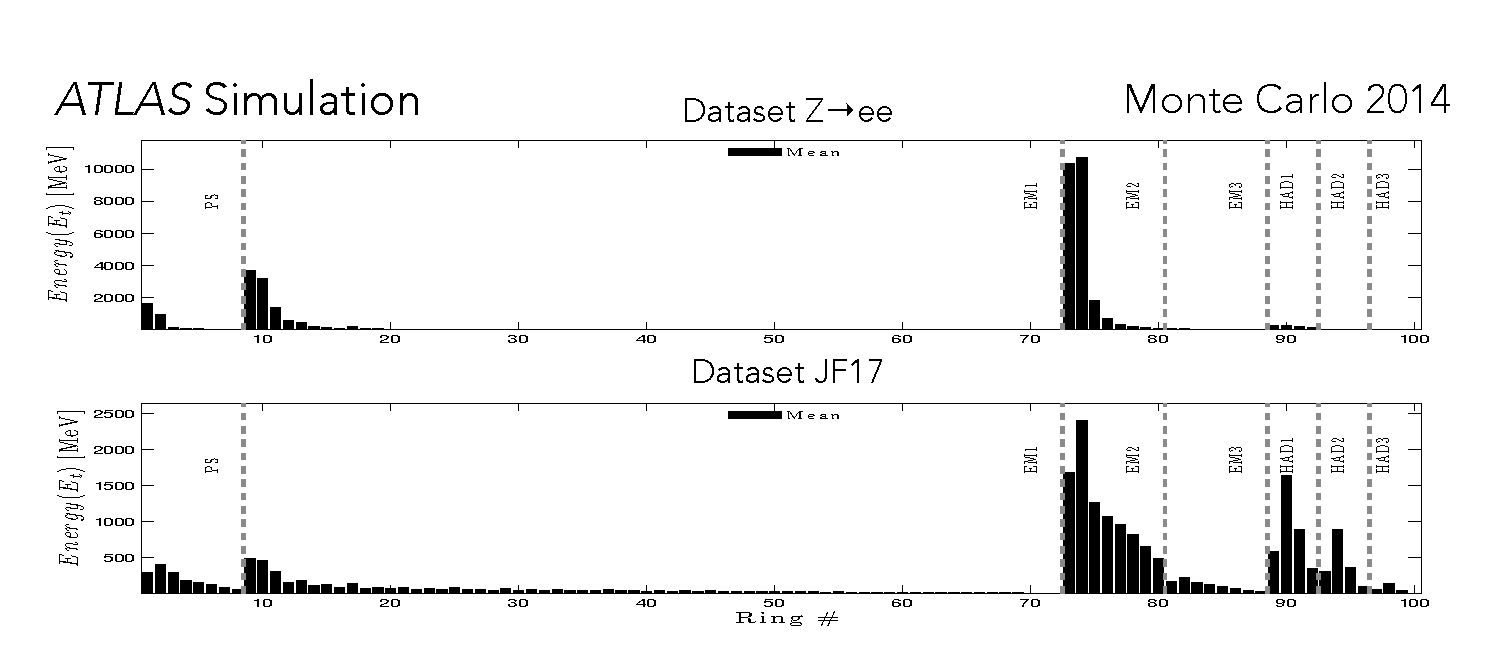
\includegraphics[width=1\textwidth]{figures/plots/ringerShape.pdf}
\caption[Perfil de energia médio para os anéis nas amostras de elétrons e jatos]
{Perfis de energia médio, medido em $MeV$, dos anéis para as amostras de elétrons (superior) e partículas hadrônicas (inferior).}
\label{fig:perfil_ringer}
\end{figure}


\section{Escolha da Rede}

O desempenho das redes de diferentes arquiteturas treinadas a partir dos dados de simulação pode ser observado
na Figura~\ref{fig:escolha_topologia}. O resultado considera a flutuação estatística estimada através do método da validação cruzada para 
os conjuntos de testes. Note que para cada configuração estão representados o valor médio e o desvio padrão dos 
50 sorteios utilizados para cada valor de eficiência (índice SP, probabilidade de detecção e falso alarme).
A escolha da topologia será dada pela observação do comportamento da flutuação do índice SP. Observe que 
o índice aumenta até 8 neurônios e após essa configuração possui um comportamento de crescimento e
decrescimento. Assim, a topologia de 8 neurônios foi selecionada como a melhor configuração a ser estudada.

\begin{figure}[h!t]
\centering
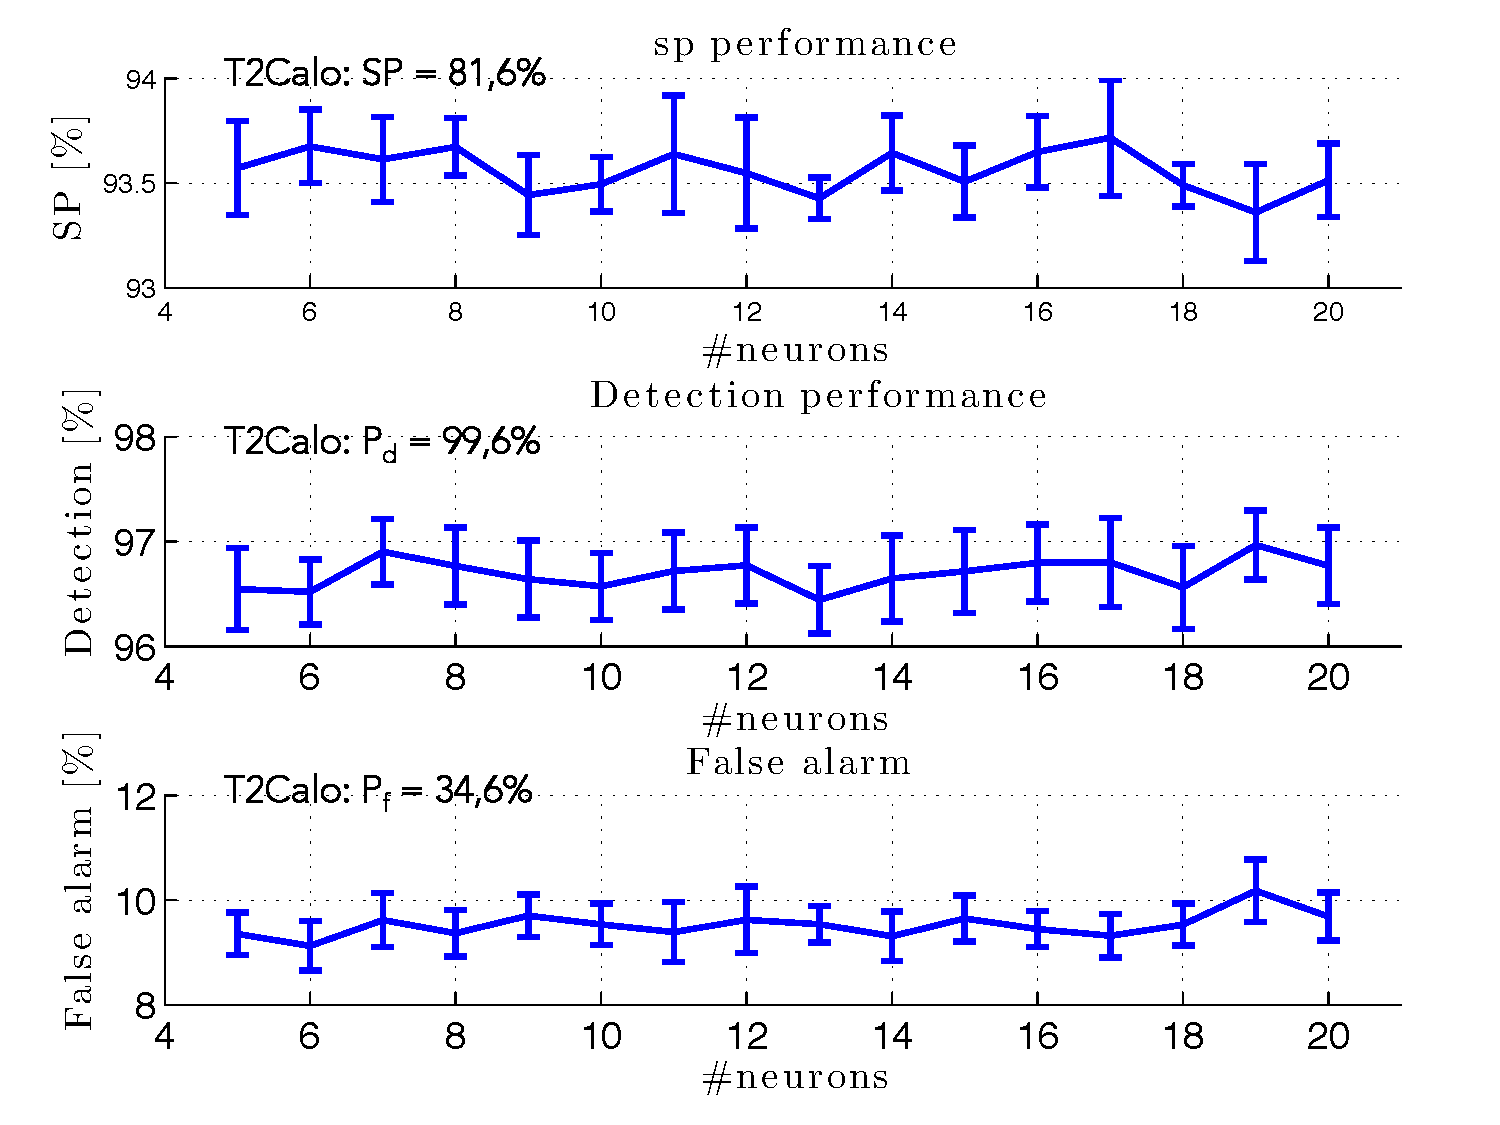
\includegraphics[width=0.7\textwidth]{figures/plots/neurons_evolution.pdf}
\caption[Flutuação estatística segundo o método de validação cruzada para cara arquitetura testada.]
{Flutuação estatística dos conjuntos de testes (50 sorteios) segundo o método da validação cruzada para cada uma das arquiteturas testadas. 
A variação do índice SP, detecção e falso alarme, com suas respectivas incertezas, para cada neurônio na camada escondida no intervalo de [5,20] neurônios,
estão representadas de cima para baixo respectivamente.}
\label{fig:escolha_topologia}
\end{figure}


Na Tabela~\ref{tab:flutuacao_validacao_cruzada}, estão representados os valores e suas respectivas incertezas
para as redes de 8 neurônios. Na última linha da tabela, estão representados os valores de eficiência do algoritmo
de referência utilizado para ajustar as redes de acordo com seu respectivo critério de parada durante o treinamento.
Na primeira linha, estão representados os valores para as redes ajustadas para valores próximos à taxa de detecção (Verde) do
algoritmo de referência. Por sua vez, a terceira linha representa os valores para as redes ajustadas para o mesmo
falso alarme (Azul) do algoritmo de referência.

\begin{table}[]
\centering
\begin{tabular}{cccc}
\hline
 & DET {[}\%{]} & SP {[}\%{]} & FA {[}\%{]} \\ \hline
ringer (pd) & \cellcolor[HTML]{9AFF99}99.6343$\pm$0.0034 & 90.4081$\pm$0.2422 & 18.3691$\pm$0.4603 \\
ringer (sp) & 96.6829$\pm$0.3708 & 93.5197$\pm$0.2046 & 9.5902$\pm$0.4719 \\
ringer (fa) & 99.9665$\pm$0.0048 & 81.7590$\pm$0.0315 & \cellcolor[HTML]{BBDAFF}34.6105$\pm$0.0566 \\ \hline
T2Calo & \cellcolor[HTML]{9AFF99}99.6349 & 81.6081 & \cellcolor[HTML]{BBDAFF}34.6124 \\ \hline
\end{tabular}
\caption[Valores de eficiência de detecção (DET), índice SP e taxa de falso alarme (FA) para a topologia escolhida.]
{Valores de eficiência de detecção (DET), índice SP e taxa de falso alarme (FA) para a topologia de 8 neurônios escolhida. 
As incertezas de cada valor foram calculadas utilizando o método de validação cruzada. Na última linha da tabela são apresentados os valores de referência 
do algoritmo T2Calo obtidos para ajustar as redes neurais nos casos de detecção e falso alarme. As redes ajustadas pelo máximo SP não possuem uma 
referência, uma vez que elas buscam o máximo índice obtido dentro de cada treinamento realizado.}
\label{tab:flutuacao_validacao_cruzada}
\end{table}

A seleção das melhores redes dentro de cada caso comparativo é obtida pelo cálculo dos valores de eficiência dos classificadores utilizando
todo o conjunto de dados disponível. Essa técnica é bastante utilizada pois durante a validação cruzada podem ocorrer casos em que um conjunto
de teste é mais fácil que outros. Assim, para evitar a polarização dos resultados, todo o conjunto de dados é utilizado para o cálculo das 
eficiências de cada uma das 50 redes treinadas referentes a topologia escolhida.


\subsection{Avaliação do Treinamento das Redes Selecionadas}

A avaliação do treinamento das melhores redes selecionadas para cada um dos critérios de ajuste estão representados nesta sub-seção.
Para os critérios de melhor índice SP e melhor taxa de detecção percebeu-se que as configurações de pesos foram obtidas do 
mesmo treinamento. Embora um treinamento retorne três possíveis configurações de pesos ajustadas, apenas as duas configurações
citadas serão utilizadas. Sendo, também, as melhores configurações obtidas dentro dos 50 treinamentos realizados para essa configuração
e critérios.

Na Figura~\ref{fig:ratevalues_sp_det}, estão representadas as curvas de evolução do treinamento para cada um dos critérios avaliados.
Para melhorar a representação gráfica, o falso alarme foi representado como a capacidade de identificação de eventos da classe de jatos. 
Assim, quanto mais próximo de '1' melhor será a rejeição do classificador aos jatos.
As épocas onde ocorreram as melhores configurações de pesos para cada um dos casos estão marcadas em cada uma das curvas.
Vale ressaltar que o treinamento só é paralisado após um determinado número de épocas ser atingido depois do último critério de parada ter sido
habilitado. Assim, em um único treinamento são extraídos três configurações de pesos referentes a cada um dos casos.
Na Figura~\ref{fig:mse_sp_det}, está representada a evolução do \acrshort{mse} para os conjuntos de treino e teste.

\begin{figure}[ht!]
    \begin{center}
        \subfigure[A evolução das curvas de detecção (Preto),  Falso Alarme (Azul) e o índice SP (Magenta) para o treinamento selecionado.]
         {
            \label{fig:ratevalues_sp_det}
            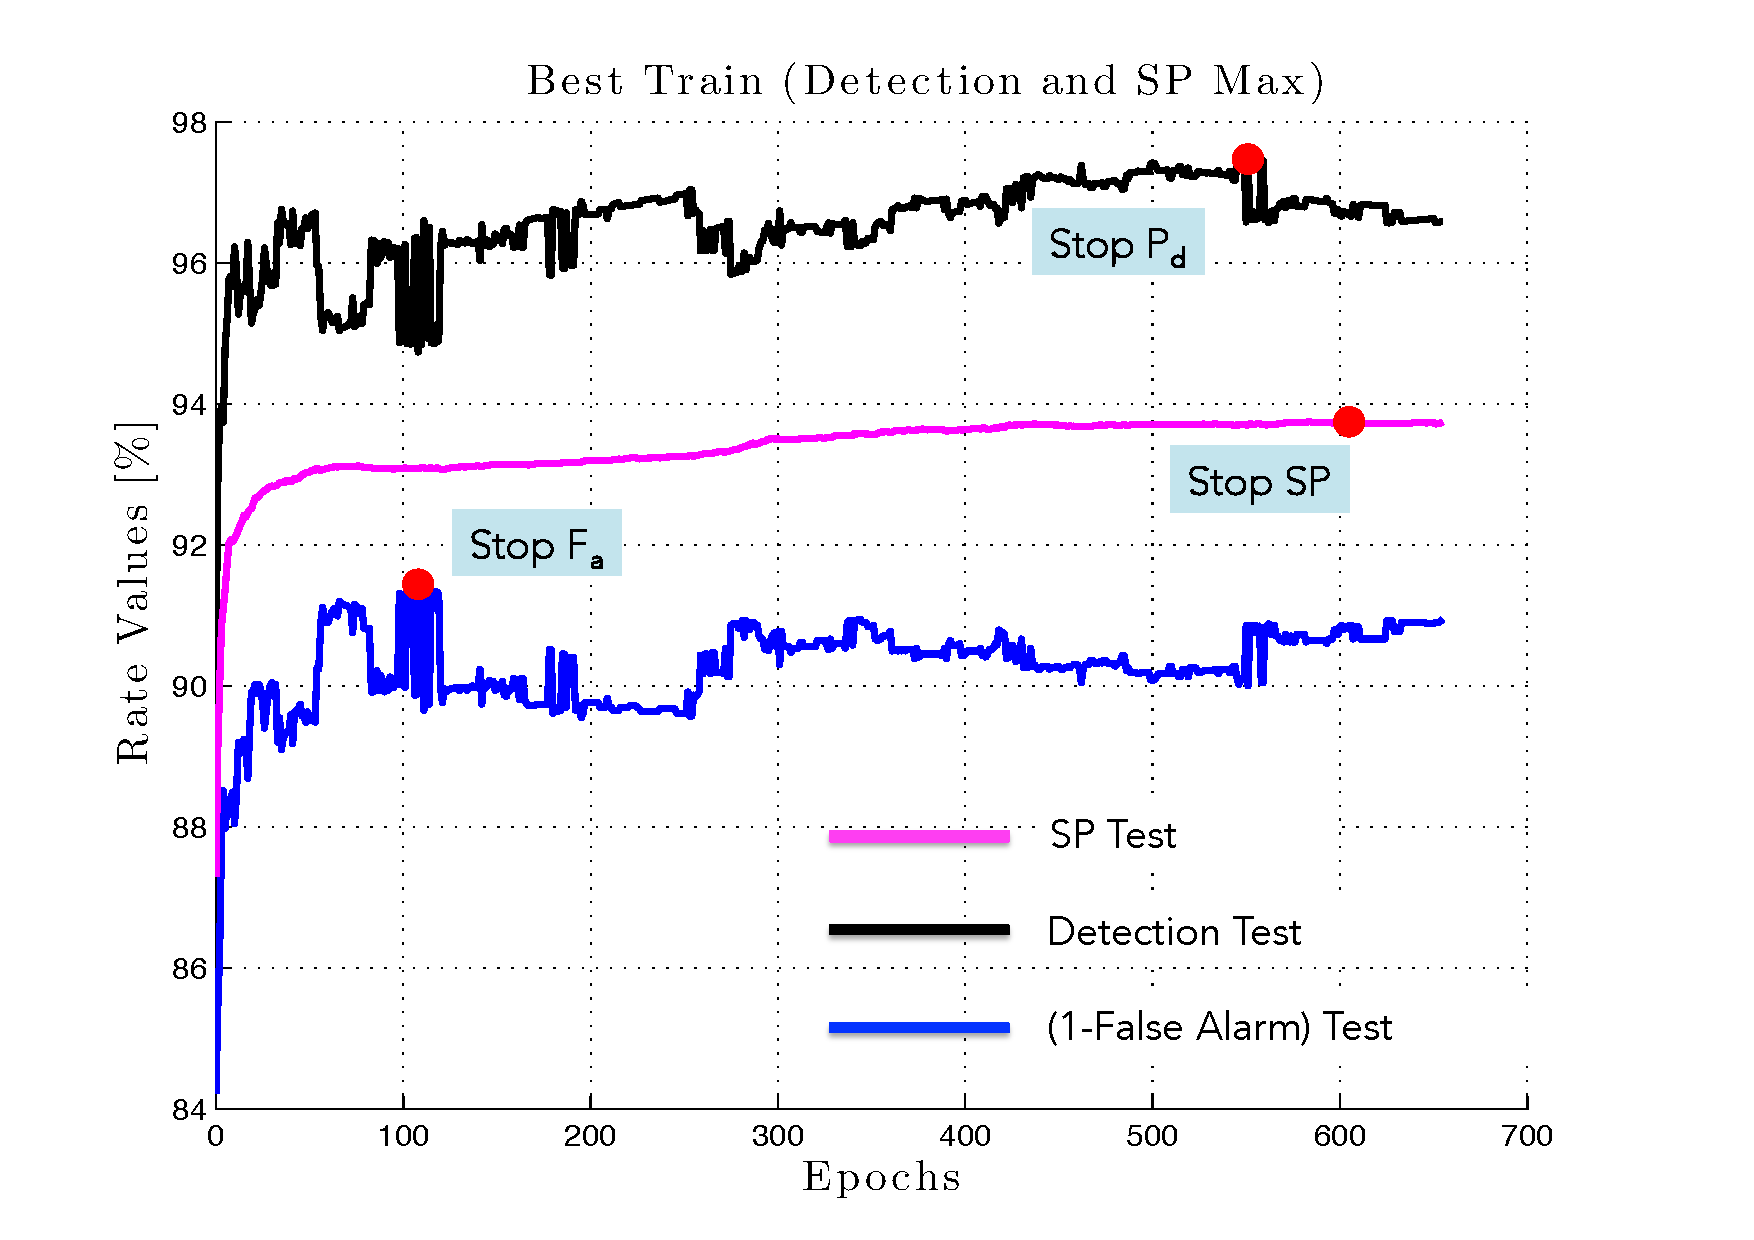
\includegraphics[width=0.46\textwidth]{figures/plots/ratevalues_evolution_sp_det.pdf}
        }\hspace{0.02\textwidth}
        \subfigure[As curvas de evolução do \gls{mse} para os conjuntos de treino e teste.]
        {
            \label{fig:mse_sp_det}
            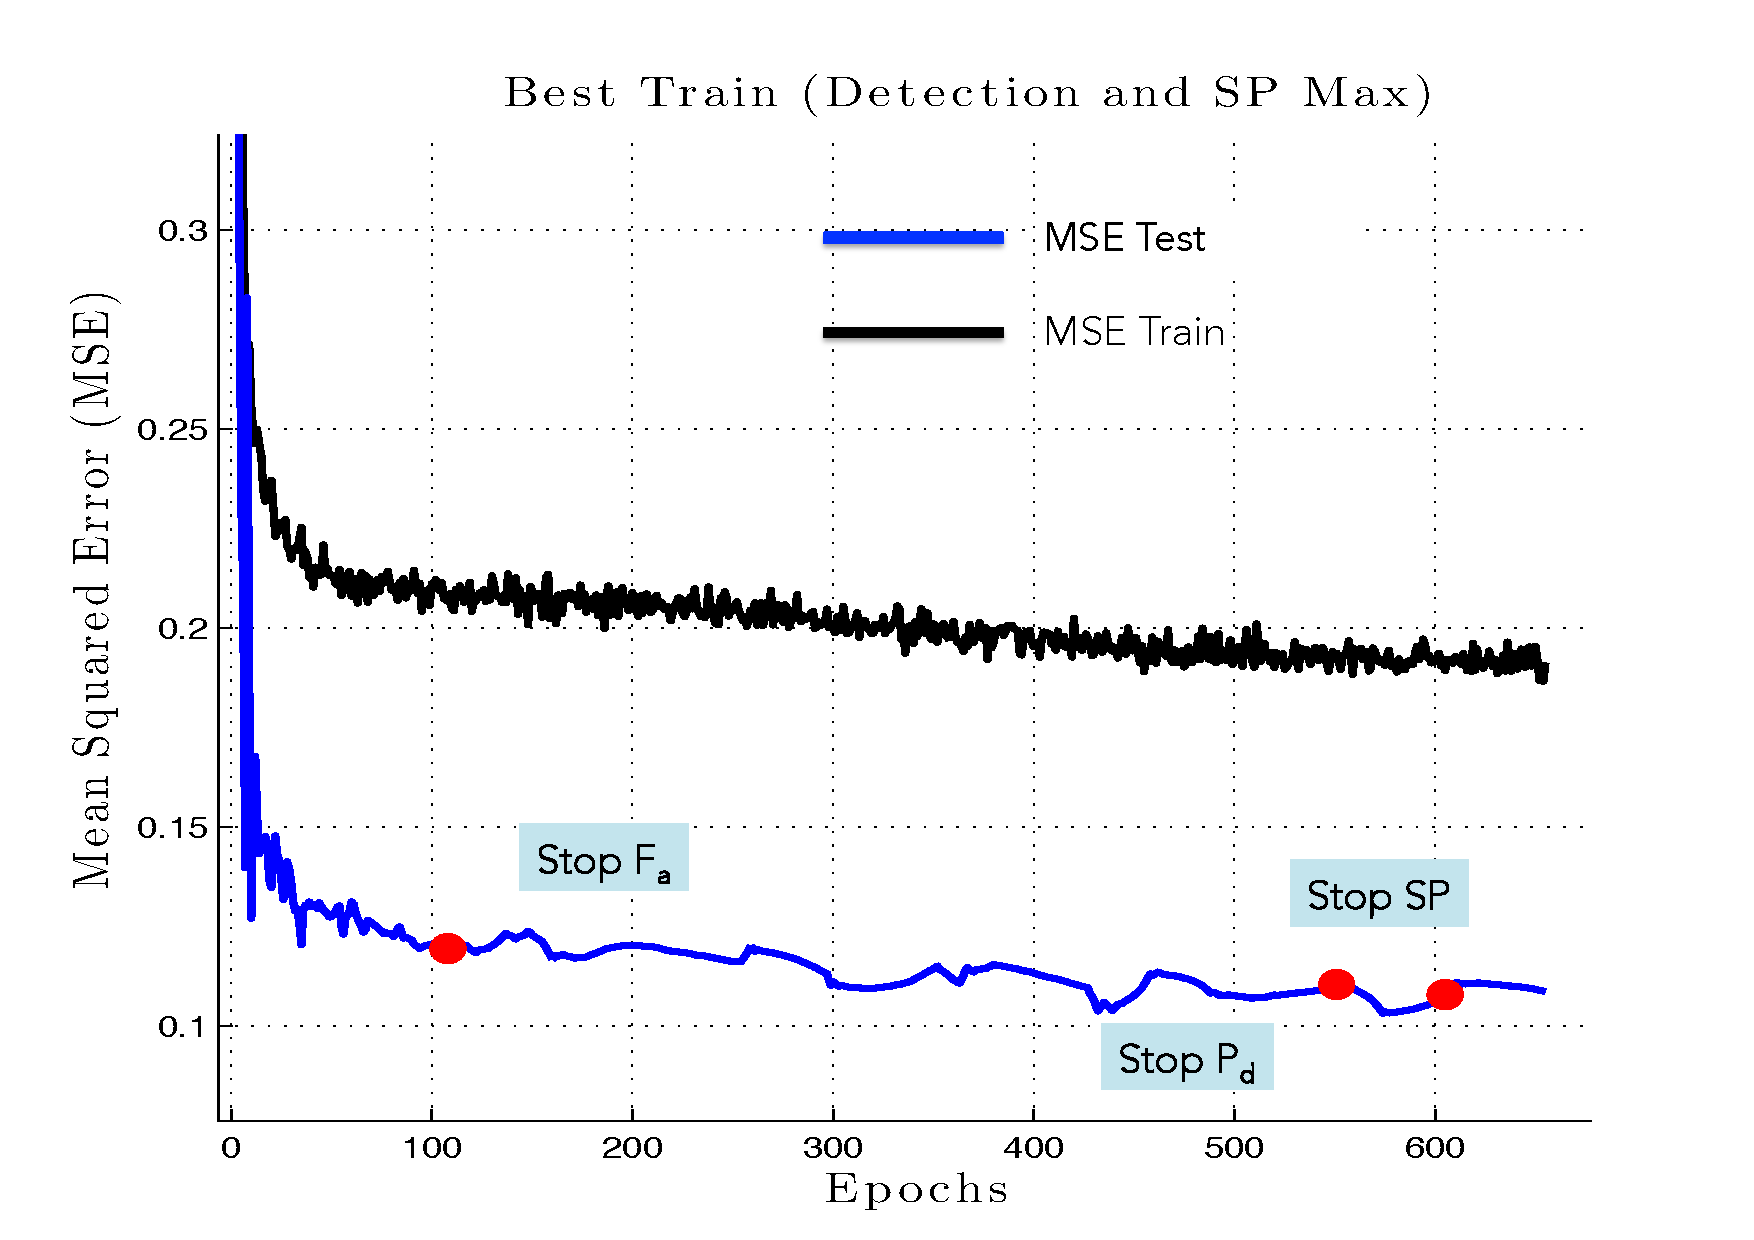
\includegraphics[width=0.46\textwidth]{figures/plots/mse_evolution_sp_det.pdf}
        }\\ 
    \end{center}
    \caption[As curvas de treinamento para as redes selecionadas pelos critérios de melhor SP e detecção.]{
    As curvas de treinamento para as redes selecionadas pelos critérios de melhor SP e detecção.}
\end{figure}

Entretanto, as Figuras~\ref{fig:ratevalues_fa} e~\ref{fig:mse_fa} representam a evolução das curvas de eficiência e \gls{mse}
ao longo do número de épocas para o treinamento selecionado com ajustes pelo falso alarme. É possível notar que nesse
treinamento, o número máximo de épocas atingidos foi menor que no caso anterior.


\begin{figure}[ht!]

    \begin{center}
    
        \subfigure[A evolução das curvas de detecção (Preto),  Falso Alarme (Azul) e o índice SP (Magenta) para o treinamento selecionado.]
         {
            \label{fig:ratevalues_fa}
            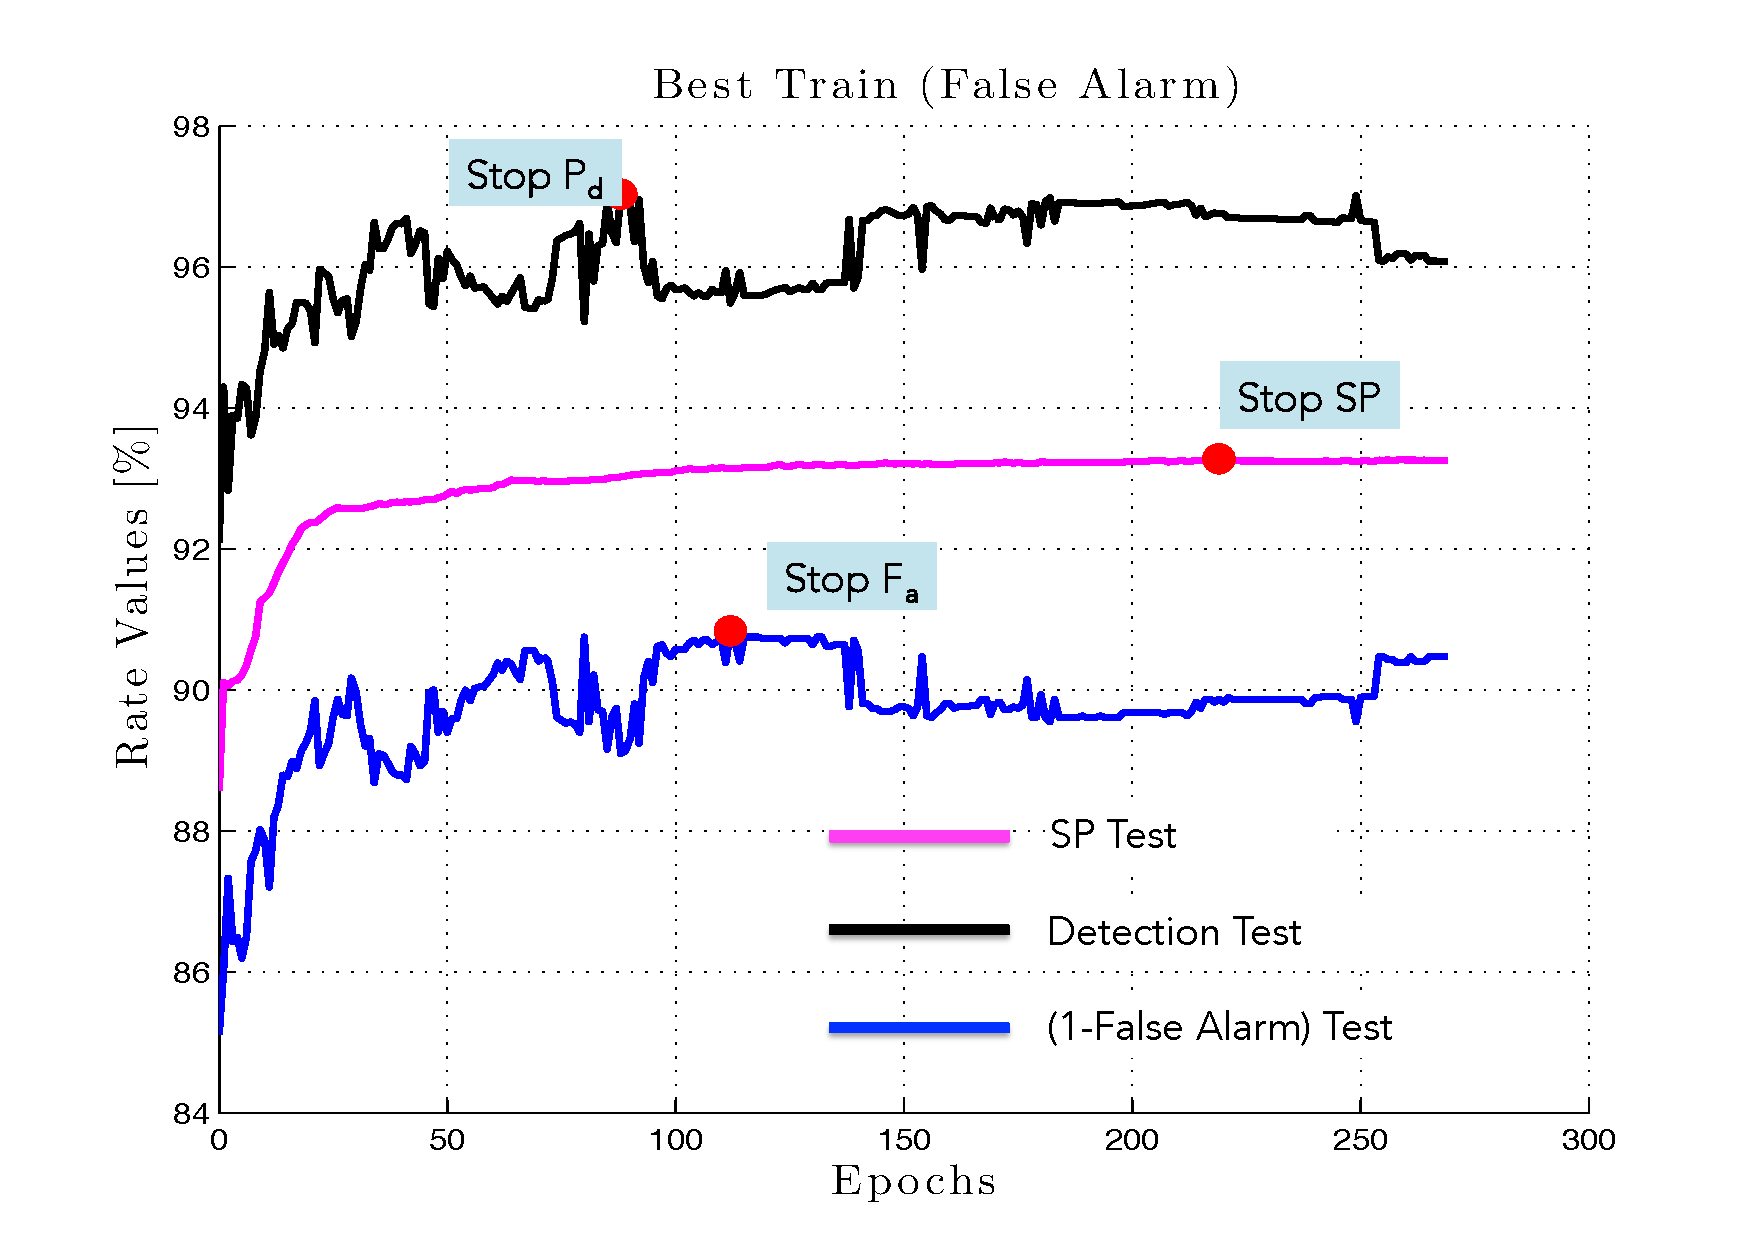
\includegraphics[width=0.46\textwidth]{figures/plots/ratevalues_evolution_fa.pdf}
        }\hspace{0.02\textwidth}
        \subfigure[As curvas de treinamento para as redes selecionadas pelos critérios de melhor SP e detecção.]
        {
            \label{fig:mse_fa}
            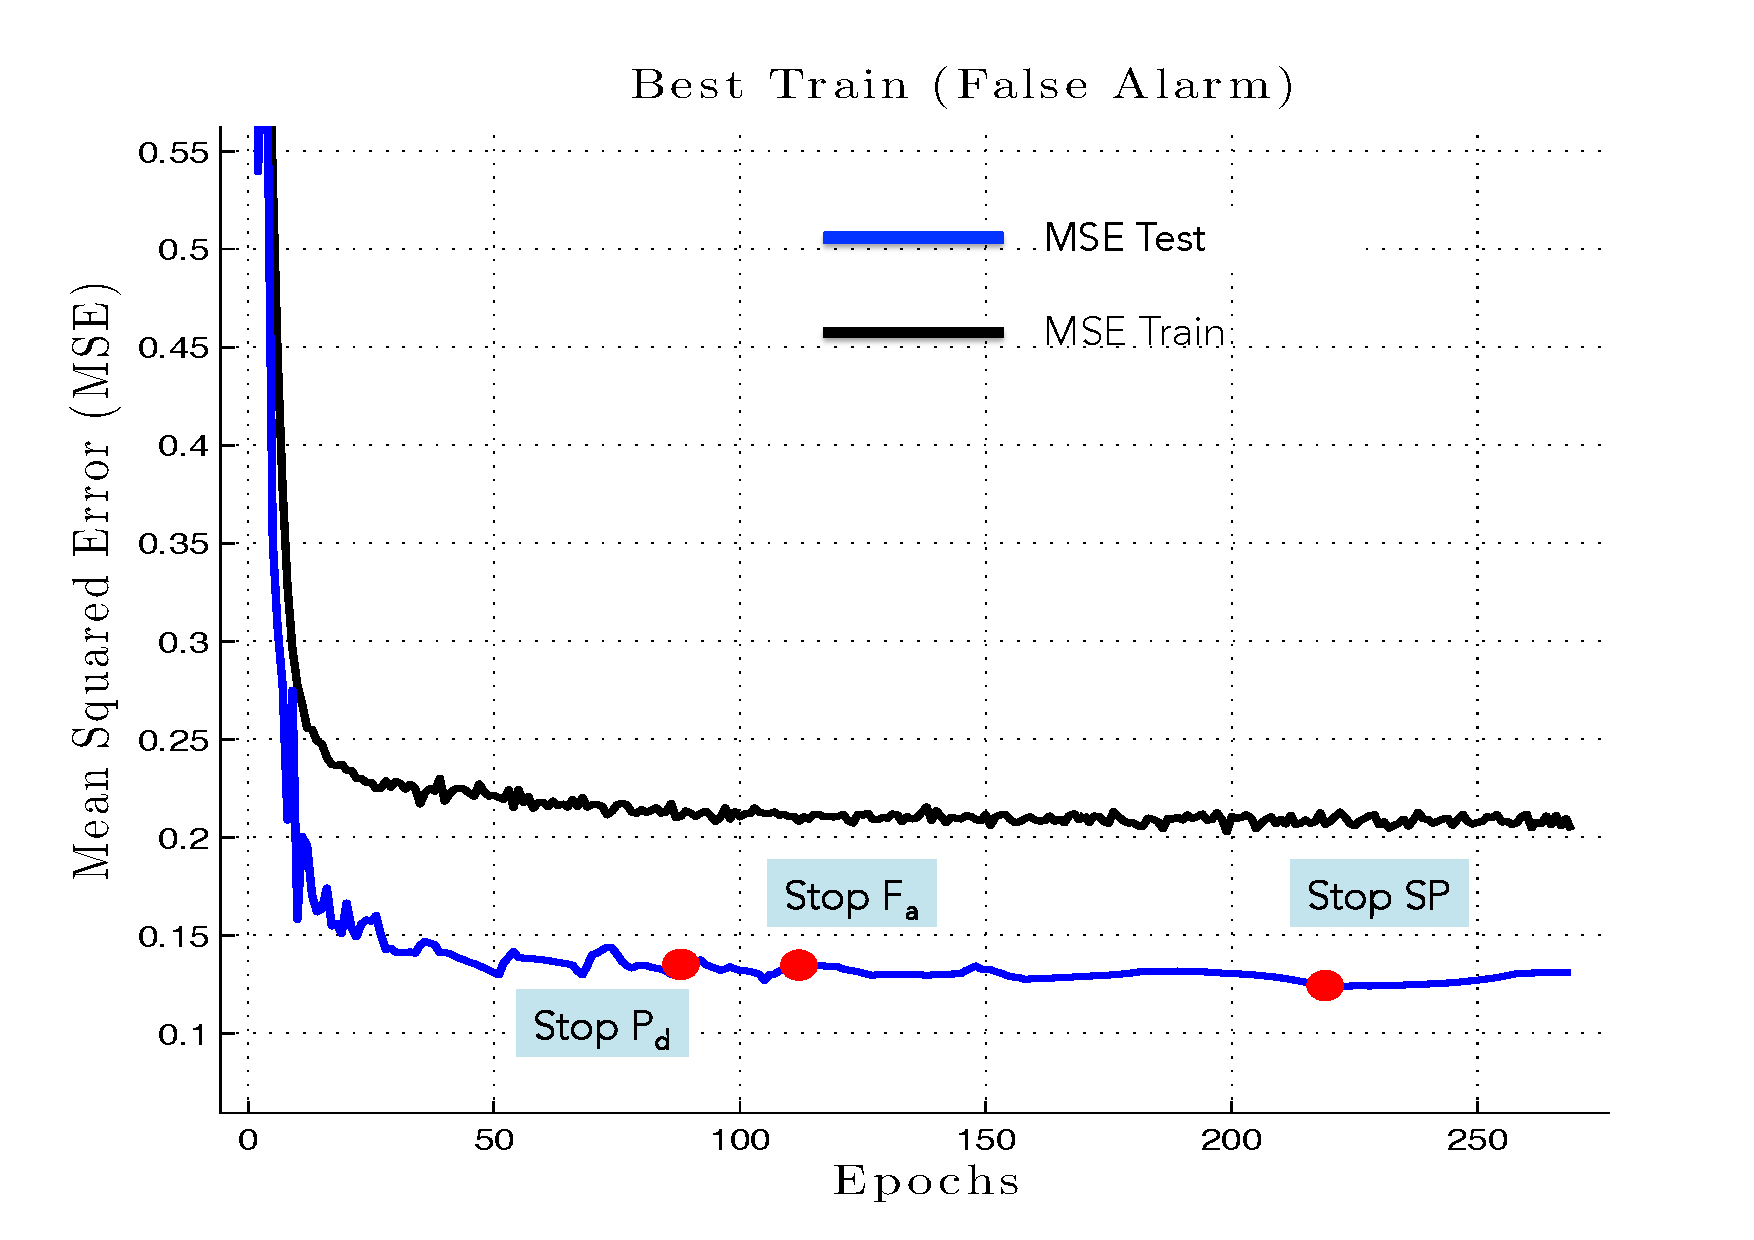
\includegraphics[width=0.46\textwidth]{figures/plots/mse_evolution_fa.pdf}
        }\\ 

    \end{center}
    \caption[As curvas de treinamento para a rede selecionada pelo critério de melhor falso alarme.]{
    As curvas de treinamento para a rede selecionada pelo critério de melhor falso alarme.}

\end{figure}



%\newpage
A Figura~\ref{fig:roc} apresenta a curva \gls{roc} para os classificadores selecionados para cada um dos critérios de ajustes
utilizados. O ponto de operação do algoritmo de referência de cada um dos ajustes também é mostrado. Graficamente,
percebe-se que para uma mesma taxa de detecção do algoritmo de referência de $99,6\%$, o classificador selecionado
para operar nessa faixa possui um falso alarme de $18,3\%$. Representando, assim, uma redução por um fator de $\sim2$ 
na taxa de falso alarme


Assim, levando em consideração que o problema está sendo aplicado em um ambiente de filtragem \textit{online} e que a 
probabilidade de detecção dos eventos é extremamente crítica nessas aplicações, foi selecionado a rede cuja taxa de
detecção foi ajustada pela do algoritmo de referência. Essa estratégia, embora mantenha a taxa de detecção, irá reduzir a
quantidade de eventos que não são interessantes para a física em \textit{triggers} superiores. Reduzindo, assim, por exemplo, o 
número de vezes que os algoritmos mais complexos, como o \textit{tracker}, serão aplicados na cadeia de \textit{trigger}.

\begin{figure}[h!t]
\centering
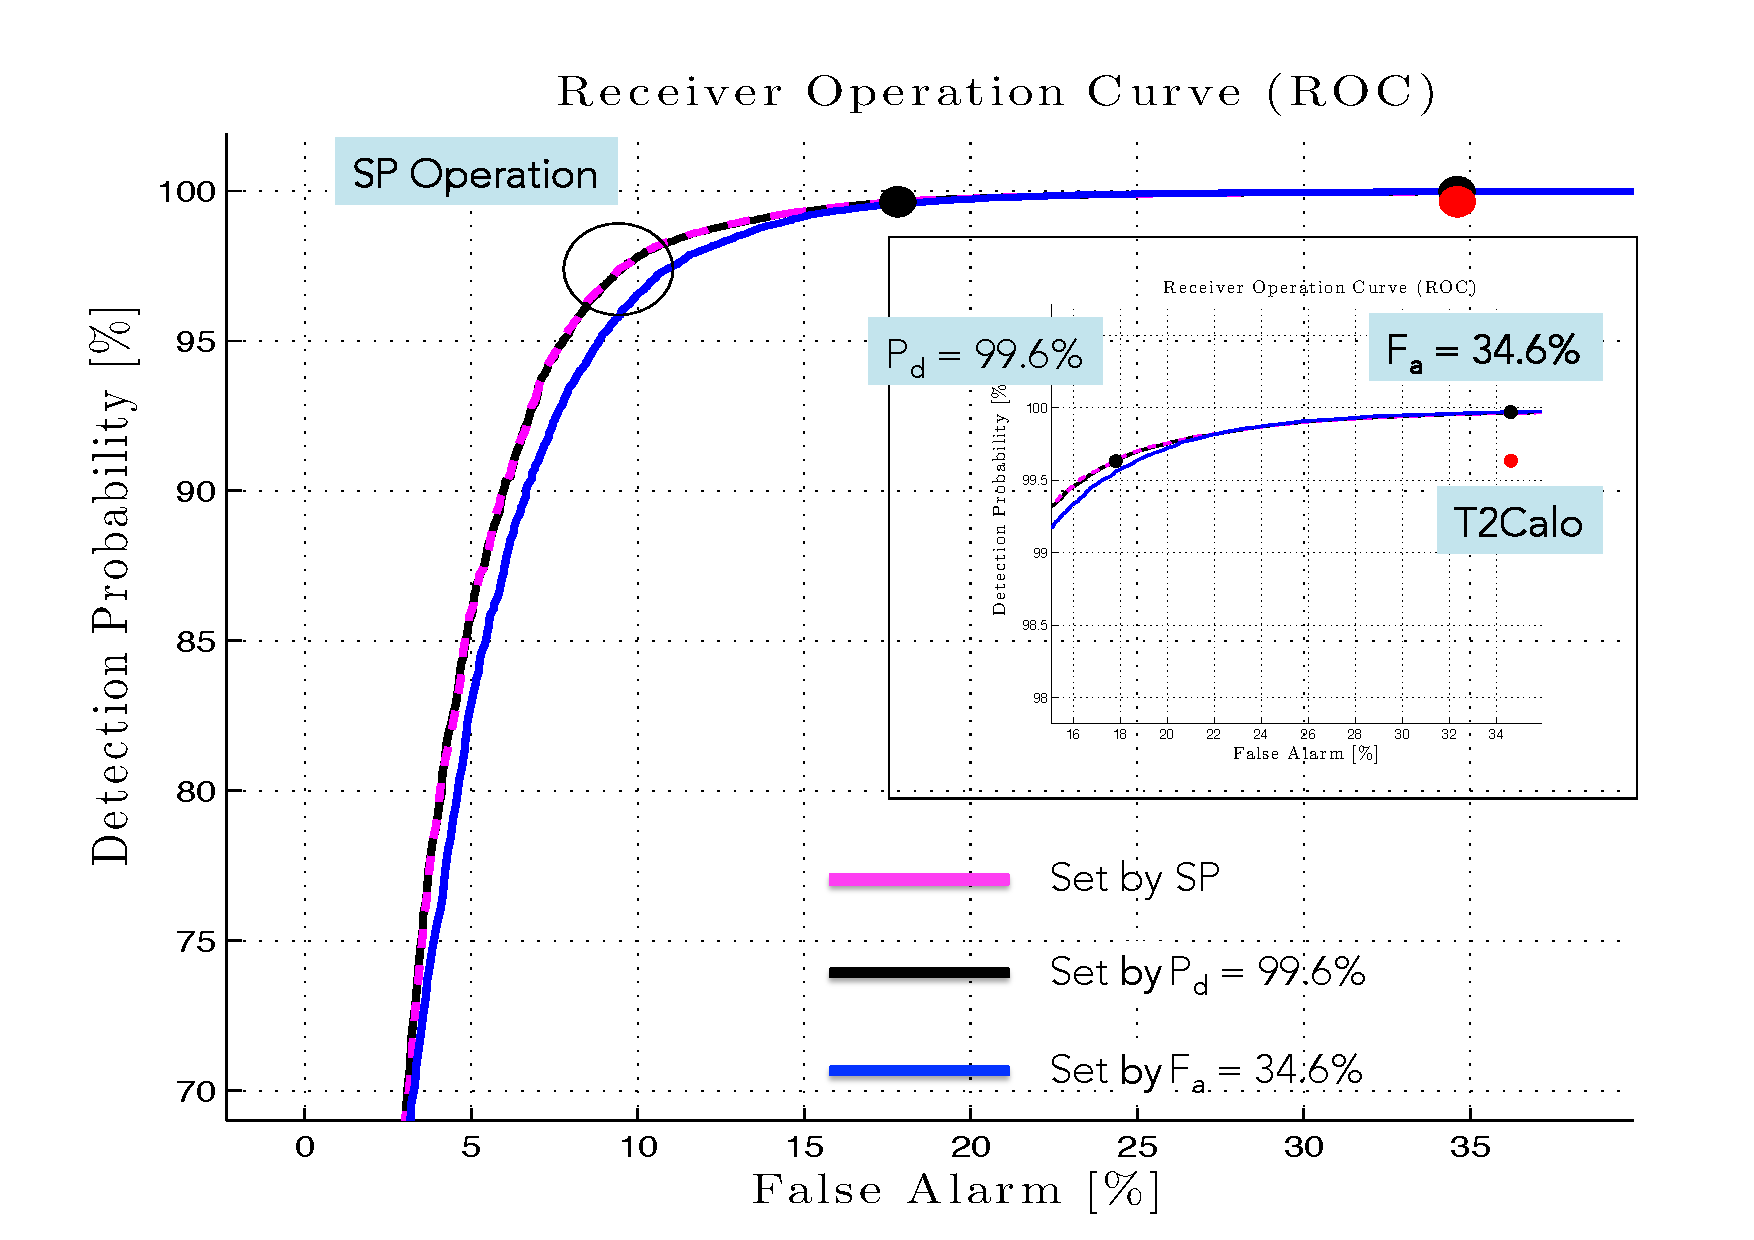
\includegraphics[width=0.7\textwidth]{figures/plots/roc.pdf}
\caption[Curva \gls{roc}]{Curva \gls{roc} e os pontos de operações ajustados para cada um dos discriminadores selecionados.}
\label{fig:roc}
\end{figure}



\section{Eficiências pelo Método de \textit{Tag-and-Probe}}

O classificador ajustado para operar com aproximadamente a mesma probabilidade de detecção do algoritmo de referência foi 
utilizado para emular a resposta do \textit{trigger} dentro do ambiente de simulação da colaboração.  
Nesta seção, serão apresentados os resultados de eficiência dos algoritmos avaliados com amostras de eventos gerados
pelo algoritmo de \textit{tag-and-probe} oficial do grupo $e/\gamma$.

Os pares gerados pelo algoritmo de \textit{tag-and-probe} foram gerados pelo conjunto de amostras do decaimento do $Z\rightarrow ee$
obtidos por simulação de Monte Carlo. Assim, as eficiências do \textit{trigger} na etapa de calorimetria rápida foram calculadas
para a \textit{chain} de referência e a nova proposta. A eficiência do método é dada pelo número
de \textit{probes} aceitos pelo algoritmo de hipótese testado dividido pelo número total de pares formados pelo método. A Figura~\ref{fig:tap_et}
apresenta as eficiência do \textit{trigger} em função da variação de energia para as respectivas \textit{chains}.

\begin{figure}[h!t]
\centering
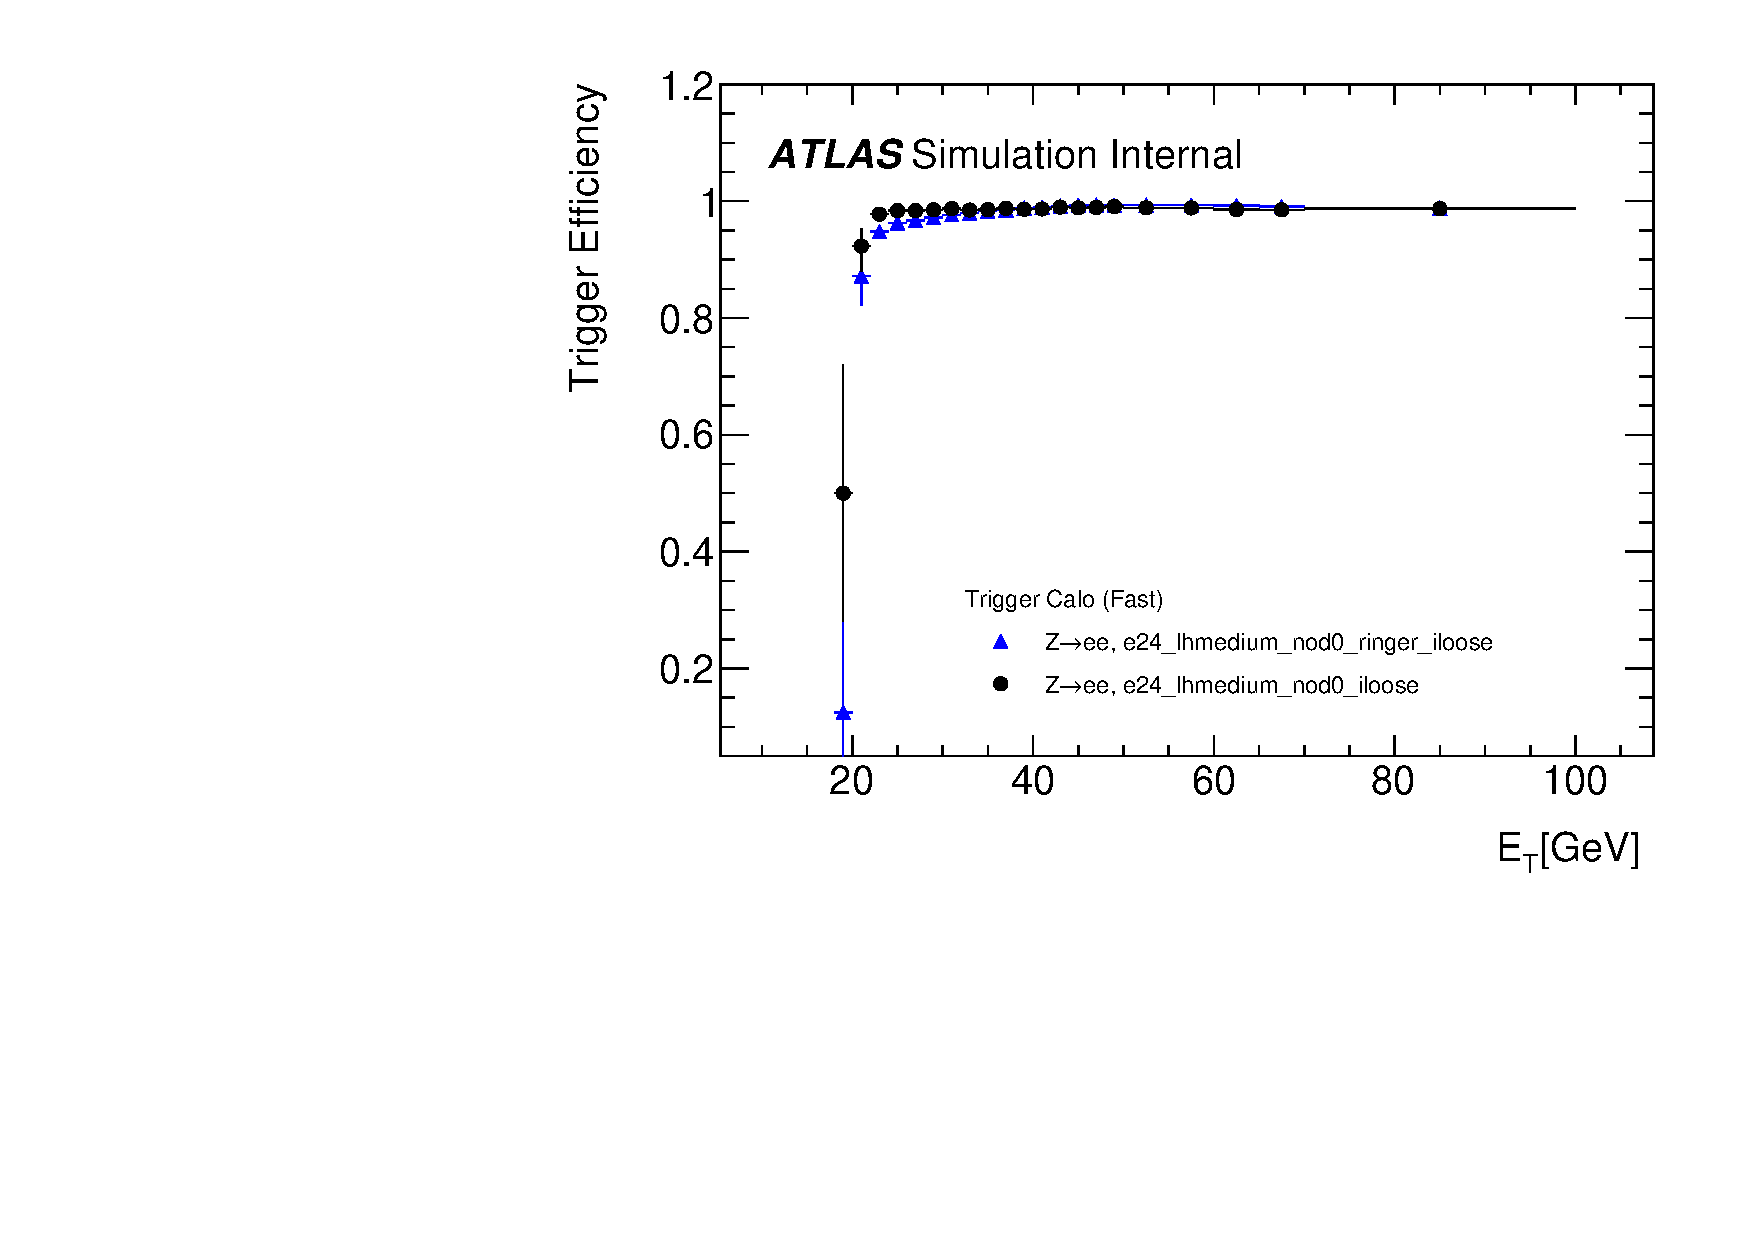
\includegraphics[width=0.6\textwidth]{figures/plots/plot_e24_lhmedium_hlt_eff_et_tap.pdf}
\caption[As eficiências do método de \textit{tag-and-probe} em função da energia em $GeV$.]{
As eficiências do método de \textit{tag-and-probe} em função da energia em $GeV$ para cada uma das \textit{chains} listadas.}
\label{fig:tap_et}
\end{figure}


Para as duas curvas de eficiência em função da energia, note que a subida da \textit{chain} do \textit{ringer} é mais lenta que o algoritmo de referência.
Esse efeito é atribuido ao ajuste dos cortes de aceitação nessa região. No caso, o algoritmo de referência possui diferentes cortes em função
da faixa de energia do evento. Diferentemente do proposto, que ajusta o limiar de corte do classificador olhando para toda
a faixa de energia.  A Figura~\ref{fig:tap_eta} mostra a eficiência de detecção dos \textit{probes} em função da região em $\eta$ no detector.  
Novamente, o algoritmo de referência também possui diferentes cortes para cada região do detector. 

\begin{figure}[h!t]
\centering
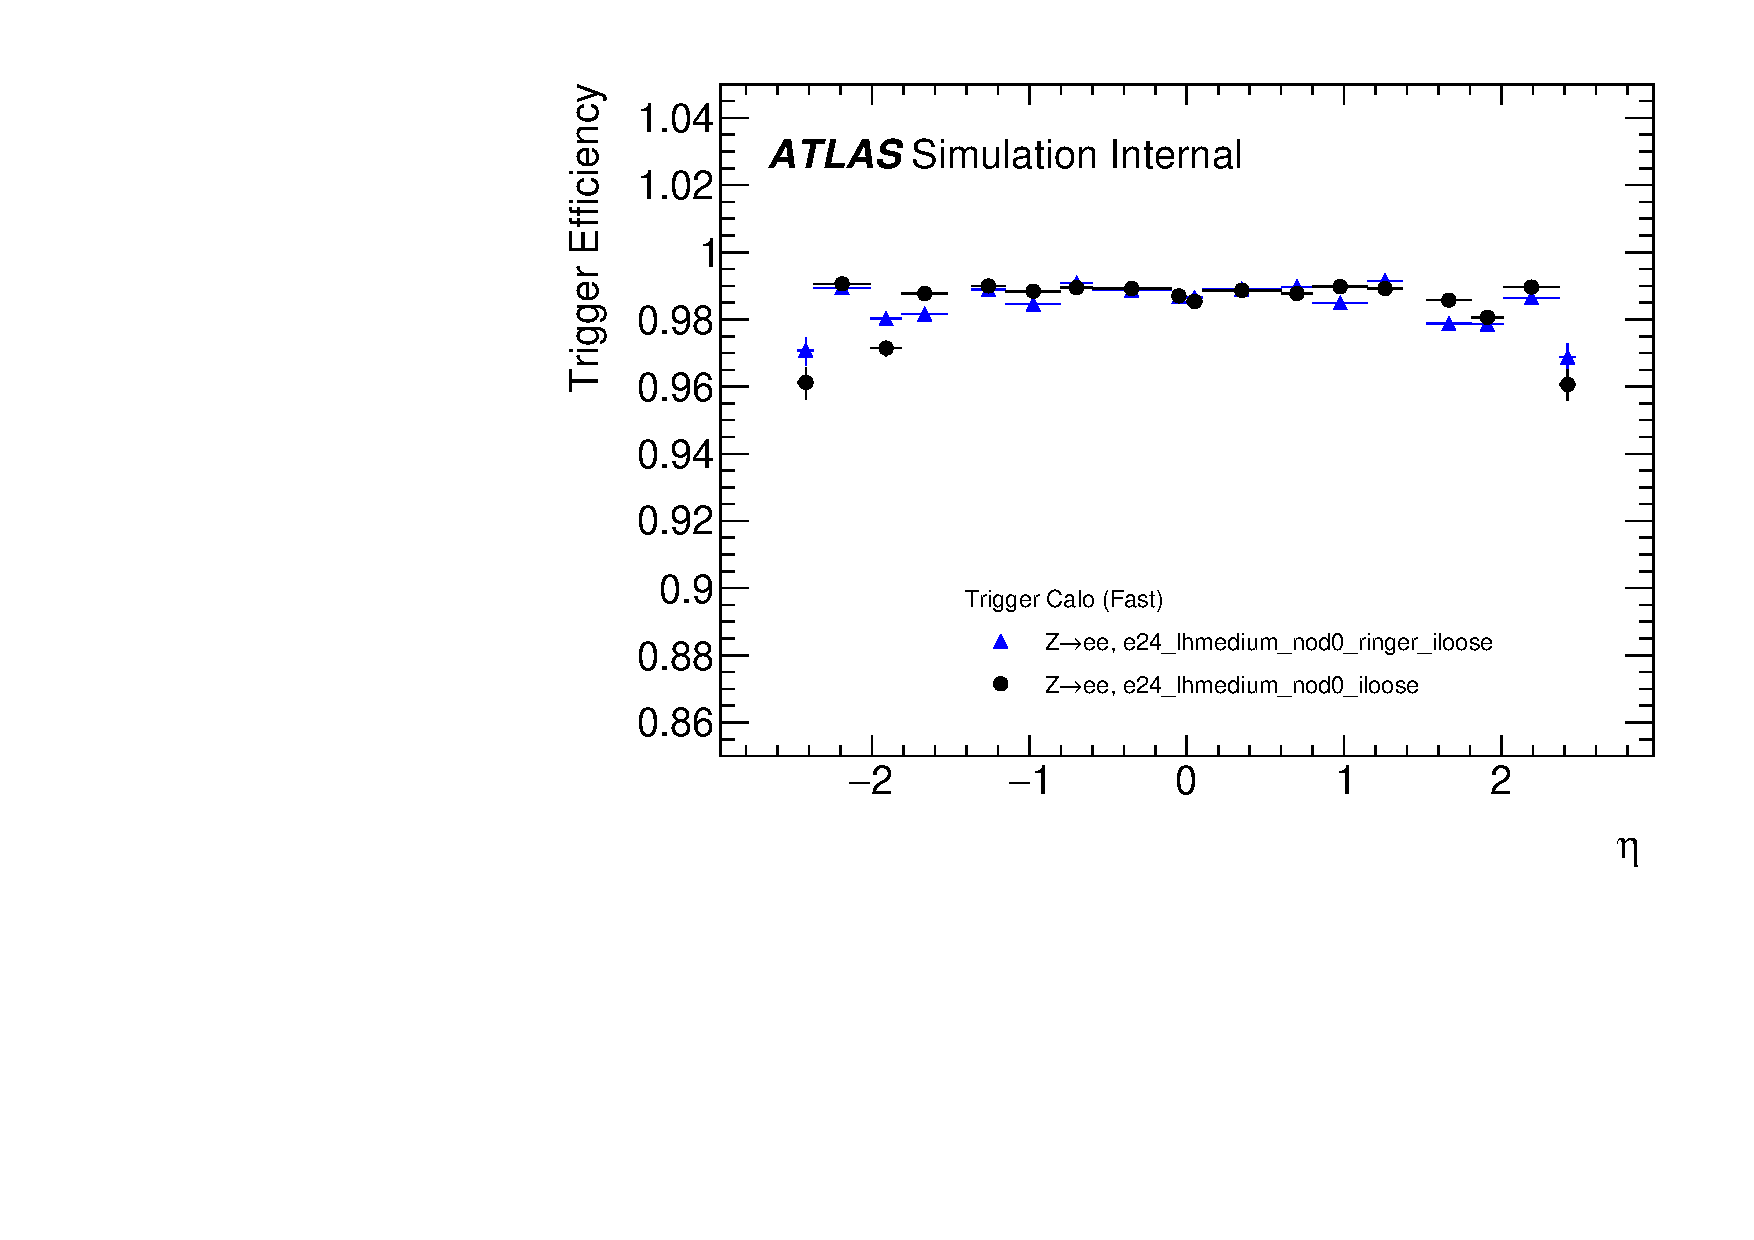
\includegraphics[width=0.6\textwidth]{figures/plots/plot_e24_lhmedium_hlt_eff_eta_tap.pdf}
\caption[As eficiências do método de \textit{tag-and-probe} em função de $\eta$.]{
As eficiências do método de \textit{tag-and-probe} em função de $\eta$ para cada uma das \textit{chains} listadas}
\label{fig:tap_eta}
\end{figure}

\newpage
Por fim, a Tabela~\ref{tab:tap_effs} mostra o resultado das eficiências das duas \textit{chains} para o método de \textit{tag-and-probe}.
Em conjunto, também foi adicionado os valores de falso alarme para os dois algoritmos utilizando todo o conjunto de dados de jatos. 
Como o valor de detecção do \textit{Neural Ringer} foi ajustado para obter valores de detecção, próximos do algoritmo de referência, então 
a comparação fica a critério da avaliação do falso alarme. Nesse caso, o \textit{Neural Ringer} obteve uma redução com um fator de $\sim2$ no conjunto de jatos.

\begin{table}[h] %\scriptsize
\centering
\begin{tabular}{ccc}
\hline
\hline
\textit{Fast Calorimeter step} & DET $T\&P$ {[}\%{]} & FA {[}\%{]} \\ \hline
e24\_lhmedium\_nod0\_iloose & \cellcolor[HTML]{FFFFFF}98.7221 & \cellcolor[HTML]{FFFFFF}{\color[HTML]{FE0000} 17.8995} \\ 
e24\_lhmedium\_nod0\_ringer\_iloose & \cellcolor[HTML]{FFFFFF}98.6269 & \cellcolor[HTML]{FFFFFF}{\color[HTML]{FE0000} 34.6124} \\ \hline  \hline
\end{tabular}
\caption[As eficiências de detecção pelo método de \textit{tag-and-probe} e falsos alarmes obtidos para as duas \textit{chains} listadas.]{
As eficiências de detecção pelo método de \textit{tag-and-probe} e falsos alarme obtidos para as duas \textit{chains} listadas.}
\label{tab:tap_effs}
\end{table}

A redução de praticamente a metade do falso alarme logo no primeiro algoritmo de hipótese do \textit{trigger} de alto nível
reduz pela metade o número de vezes de chamadas dos algoritmos de hipótese posteriores. Embora esses algoritmos
possuam a capacidade de eliminar os mesmos eventos rejeitados pelo \textit{Neural Ringer}, sua aplicação requer um tempo 
de latência maior e análises mais refinadas para inferir a mesma resposta que um simples classificador multi-camadas
apresentado como proposta para colaboração. Assim, a implementação de um sistema altamente eficiente combinado
com uma extração de características, no caso os anéis, mais completa resultou em uma classificação mais eficiente
que o algoritmo de referência utilizado como comparativo 



